\documentclass[a4paper,10pt,oneside, fleqn]{article}
% Druckbereich: \areaset[BCOR]{textwidth}{textheight}
% BCOR ist "Binding Correction", also wieviel Innenrand verloren geht
% A4 hat 297mm x 210mm
% wenn keine Marginalien, dann ist Breite 15cm vielleicht besser
%\areaset[0cm]{15cm}{25cm}


\usepackage[english,mt]{ethidsc}    % deutsche Übersetzungen und Wortumbrüche
\usepackage{mcode}
\usepackage{subfigure}

   
% Page header (don't change)____________________________________________________
\setlength{\parindent}{0em}                 % Disable parindent
\rhead[\nouppercase{\rightmark}]{\thepage}  % Special headings
\lhead[\thepage]{\nouppercase{\leftmark}}   % Special headings
\cfoot{} 
 
%%% hier können noch viel viel mehr Einstellungen kommen

%%% Title page
\title{To be determined}

\studentA{Jennifer Studer}
\ethidA{16-915-928}
\semesterA{2}
\emailA{studerje@student.ethz.ch}

\supervision{Christian Tschudi\\ Hans Martin Schmid}
\date{\today}

 
%%%% hier beginnt der Inhalt %%%%%%%%%%%%%%%%%%%%%%%%%%%%%%%%%%%%%%%%%%%%%%%%
\begin{document}

\maketitle

\pagestyle{fancy}               	% Fancy headings
\pagenumbering{arabic}

\vspace*{\fill}
\begin{abstract}

\end{abstract}
\vspace*{\fill}
\newpage

\tableofcontents
\newpage

\section{Introduction}
The question whether there is life on other planets then earth has always been of interest for humans. To find an answer to this question scientist try to find possible habitable planets. Since it is easier to search for life which is already known an approach is to search for earth-like planets.\\
A problem in the search for habitable planets via direct imaging is mainly that it is assumed that they need to be already older, since young planets are hot and old planets are harder to detect. The temperature of a young giant planet is between $T \approx 1000$ - $2000$ K this means that it will emit mainly in the near-infrared and the contrast which is required to resolve young planets $C = F_{\mathrm{pl}}/F_{\mathrm{star}} \approx 10^{-5 \pm 1}$ \cite{Hunziker2020}. Whereas an old planet is a lot colder and the light it emits is in the visual to near-infrared, since it is caused by the scattering of the host-stars light. Therefore the contrast required to resolve an old planet is a lot smaller, namely around $C \lessapprox 10^{-7}$ \cite{Hunziker2020}.\\
With the current instruments available it is still very challenging to reach this small contrast. Therefore most planets which have been found so far, which are potentially habitable are close to our solar system and/or their host star is less luminous than our sun.\\
In order to be able to detect planets with small contrasts we can either improve our instruments and measurement methods or we can try to improve the quality of the already taken data with data analysis. In this report we are going to focus on the later. \\
In the following we are going to describe the possibility to suppress the spiders in astronomical data with the help of Fast Fourier transformation. We have four spiders in each image data which are caused by the spider arms of the telescope. These arms are the mechanical struts that hold the secondary mirror of the telescope \cite{ESOmanual}.\\
Recall that the Fourier transformation of a integrable function $f(x)$ on $\mathbb{R}^n$ is given by
\begin{equation}
	\mathfrak{F}\{f(x)\} = F(\mu) = \frac{1}{\sqrt{2\pi}^n} \int_{\mathbb{R}^n} f(x) e^{-i\mu x} dx.
\end{equation}
The inverse Fourier transform of it is
\begin{equation}
	f(x) = \frac{1}{\sqrt{2\pi}^n} \int_{\mathbb{R}^n} F(\mu) e^{i\mu x} d\mu.
\end{equation}
Important properties of the Fourier transformation and its inverse are that they are linear. This means that Fourier transform of the sum of two functions is the same as the sum of the Fourier transformation of the two function and that a scalar factor can multiplied to the Fourier transform before or after the transformation. An other important property of the Fourier transformation is that convolutions of two functions is equal to a multiplication in the Fourier space. \\
To undo a multiplication in the Fourier space is a lot easier than undoing a convolution in the image space.This means that the Fourier transformation is especially helpful, if we want to get rid of a pattern which is caused by a convolution. In our case, however, the spiders is a pattern which is added on top of the other image information. This means we need to subtract the spiders from the image. This operation is dangerous, because we need to guess the intensities caused by the spiders and by subtracting by this guess we can destroy the information below the spiders. In the Fourier space we also need to subtract the frequencies caused by the spiders. Our hope is the frequencies caused by the spiders are really different then the ones caused by the exoplanet or other interesting features. This would enable it to cut out the respective frequencies without the problem of destroying important information.\\
To compare the effect different operations have on point sources we describe in section \ref{sec:aperture_phot} how the aperture flux is calculated and we look at the aperture flux of the ghosts in the image data of HD142527. We will use the image data of HD142527 from the VLT telescope to test suppression of the spiders. HD142527 is a binary star system which is still quite young. The two stars are surrounded by a protoplanetary disk which makes the system interesting for the investigation on planet formation processes inside the protoplanetary disk \cite{HD142527}.\\
The transformation of the image data into the $r$-$\varphi$ plane is described in section \ref{sec:interpolation}, where we also investigate the effect this transformation has on the data. Then we subtract the radial intensity drop off from the transformed image as it is explained in section \ref{sec:radial_intensity}. In section \ref{sec:fourier} we take a closer look at the Fourier transformation and how the frequency plane of specific features looks like. Here we focus primarily on spider like features. After we have gained an understanding of the frequency plane we use this knowledge in section \ref{sec:suppressio} to suppress certain frequencies in order to get back an image where the spiders have vanished. We try out two different methods. In the first method we subtract the frequencies from the spider, which is the mathematical correct way. In the second method we divide by a Gaussian profile, which is mathematically wrong, but more stable then the subtraction. At the end we summarize our results in section \ref{sec:results}.\\
The scripts used for the simulations and calculations are written in python and can be found 
on GitHub, see \cite{github}.

\section{Aperture Photometry}
In order to determine the flux of different objects in astrophysics, like stars and planets, aperture photometry can be used. This method sums the counts of the pixels inside a certain aperture around the star. In our case this aperture is usually a circle. In order to account for the background noise an annulus around the aperture is taken and the mean of the summed up pixels inside the annulus is subtracted from the apertures pixels. The flux of this aperture is then given by \cite{Gisin}
\begin{equation}
	F_{ap} = F_{tot} - n_{px} \langle F_{bg} \rangle ,
\end{equation}
where $F_{tot}$ is the total flux inside the aperture (sum up the pixel values inside the aperture), $n_{px}$ is the number of pixels inside the aperture and $\langle F_{bg} \rangle$ is the mean background per pixel. This mean background per pixel is defined through the annulus and calculated from
\begin{equation}
	\langle F_{bg} \rangle = \frac{1}{m} \sum_{i=1}^{m} c_{i} ,
\end{equation}
where $m$ is the number of pixels in the annulus and $c_{i}$ the respective pixel value.
Figure \ref{fig:aperture_ex} shows an example for a possible aperture and an annulus around a star, which can be used to do an aperture photometry.
\begin{figure}[H]
	\centering
		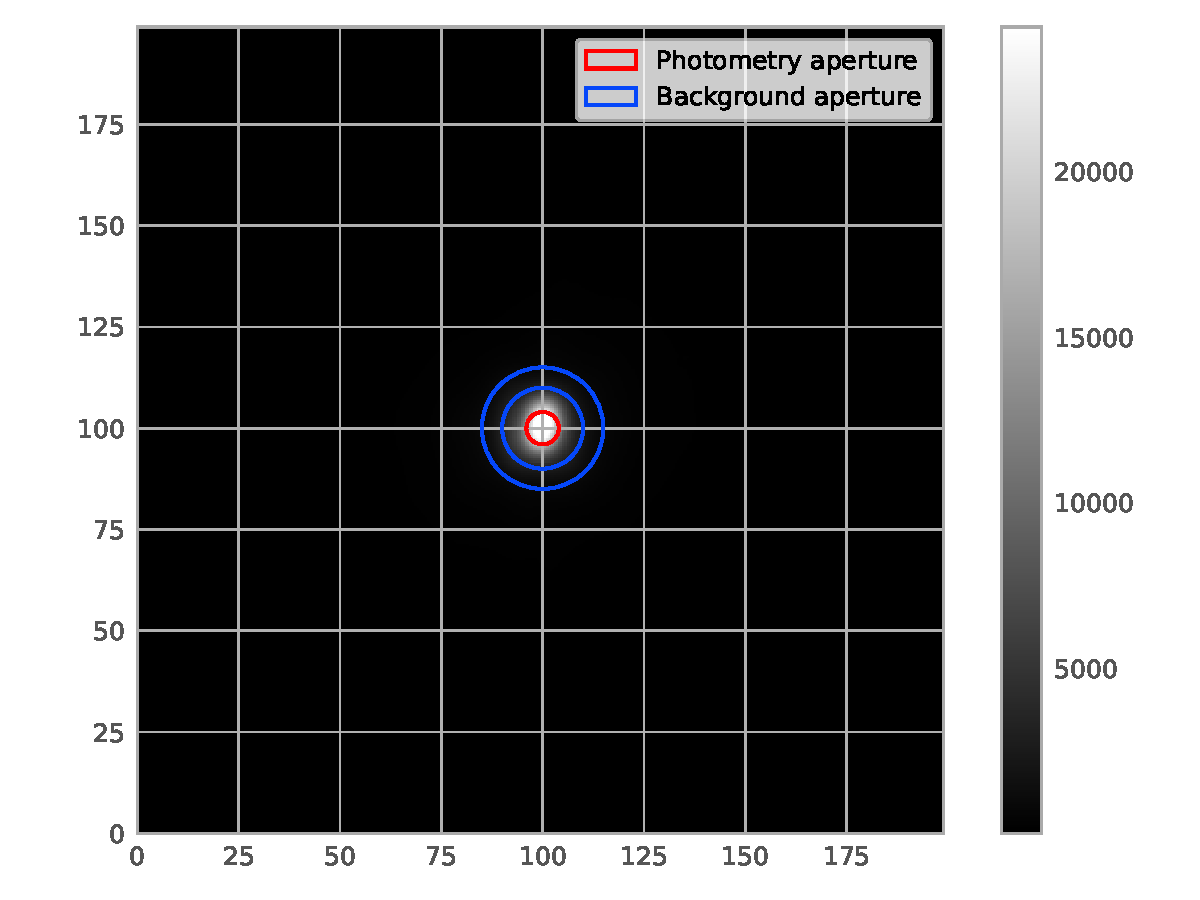
\includegraphics[width=0.9\textwidth]{pics/aperture_example.pdf}
		\caption{An aperture photometry for the star in the center, where the red circle indicates the aperture used and the two blue circles define the annulus used for the background subtraction.}
		\label{fig:aperture_ex}
\end{figure}
From the figure you can see that we chose the annulus not directly after the aperture, but this is just one way to do it. One could also choose the annulus directly after the aperture or choose a different distance between the annulus and the aperture. However the annulus should give a good approximation for the background inside the aperture and therefore it should not be too far away from the aperture. We chose a small distance between the aperture and the annulus of 4 pixels, because we wanted that as little starlight (in this case) as possible is included in the annulus. If we plot the counts per pixels which are included in a certain radius around the star, as it is done in figure \ref{fig:annulus_radi} we see that after around 10 pixels the increase is decreasing rapidly. That is where there is only little starlight left. This is also why we choose the annulus to go from a radius of 10 to 15 pixels. 
\begin{figure}[H]
	\centering
		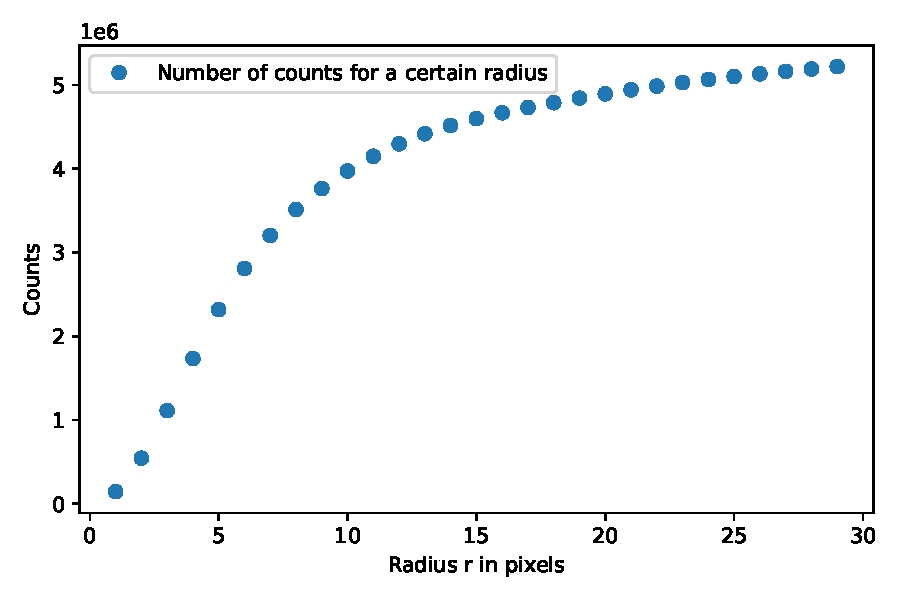
\includegraphics[width=0.8\textwidth]{pics/CountsPerRadius.pdf}
		\caption{The total flux of the star is calculated for different radii and plotted. This shows that after a radius of 10 pixels the contribution from the star is almost gone.}
		\label{fig:annulus_radi}
\end{figure}
Additionally we choose the radius of the aperture to be 6 pixels.

\subsection{Aperture photometry and ghosts}
In order to detect exoplanets one can use aperture photometry. In this subsection we are going to do these steps for the two ghosts which we have in our data from the circumstellar disk HD142527, in order to demonstrate how this could be done for an exoplanet and to learn more about ghosts.\\
A ghost is a copy of the star, which is created by the back-reflection of the star on optical components of the telescope. Figure \ref{fig:ghosts} is an image of HD142527, where the two ghosts are indicated. We see that the ghost on the top right (we will call this ghost 1) is brighter than the ghost on the bottom left (ghost 2). 
\begin{figure}[H]
	\centering
		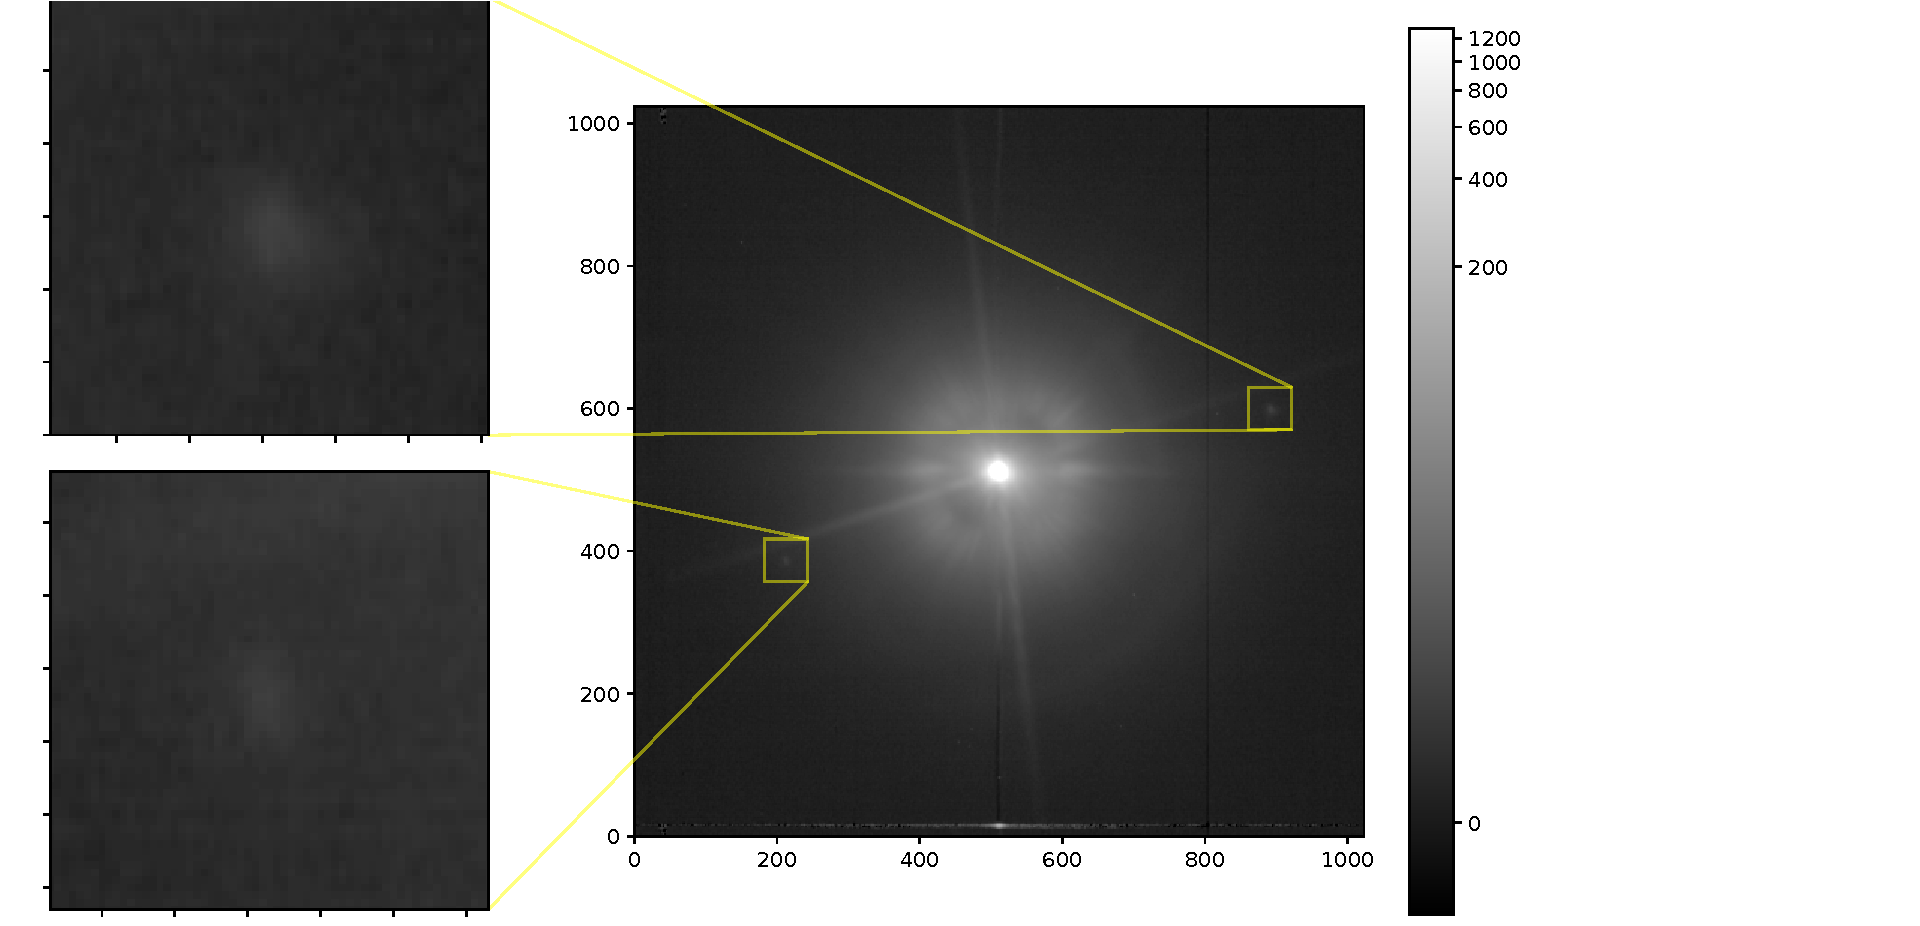
\includegraphics[width=1.3\textwidth]{pics/Ghosts.pdf}
		\caption{An image of the circumstellar disk HD142527, where the two ghosts are indicated.}
		\label{fig:ghosts}
\end{figure}
If we want to confirm the signal from our ghost or also from other objects like exoplanets, which usually can not be seen by eye, we use the signal to noise ratio $S/N$. This means we do aperture photometry for several points around the star which are at the same separation from our star as the ghost (or exoplanet etc.), as in figure \ref{fig:ap_phot_gh1}. From this we can calculate the standard deviation $\sigma$ from the mean of all aperture fluxes and the signal to noise ratio. If the signal to noise ration is larger than the standard deviation, this means that we have a source (ghost, exoplanet) at this position. 
\begin{figure}[H]
	\centering
		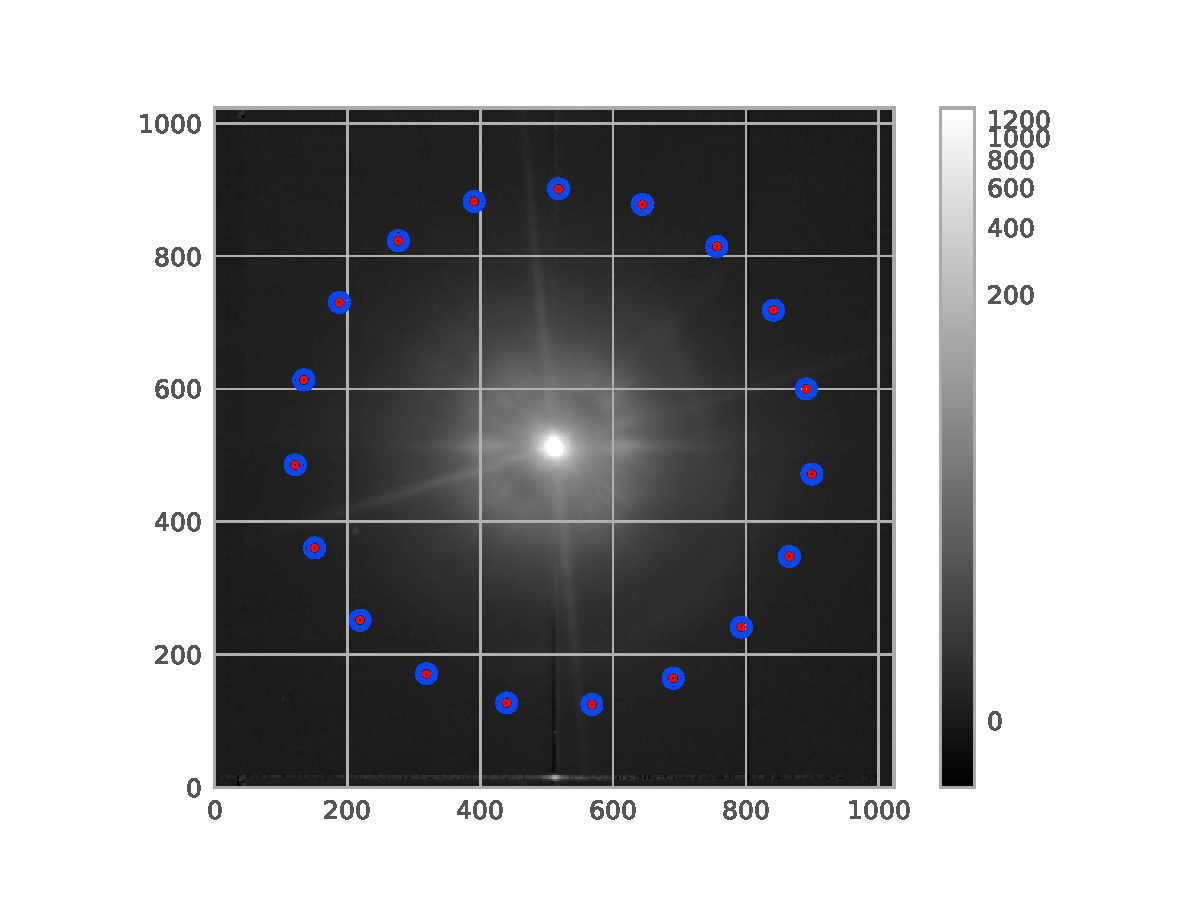
\includegraphics[width=0.9\textwidth]{pics/aperture_photometry_19_ghost1.pdf}
		\caption{In order to confirm the signal from the ghost, we do aperture photometry for several points around the star which are at the same distance from the star as the ghost. We then calculate the standard deviation of all the aperture fluxes and from there find the signal to noise of the ghost's aperture. If the signal to noise is larger than the standard deviation, the position of the ghost is confirmed.}
		\label{fig:ap_phot_gh1}
\end{figure}
The standard deviation is calculated by
\begin{equation}
	\sigma = \sqrt{\frac{1}{k-2} \sum_{ap=2}^{k} (F_{ap} - F_{mean})^2} ,
\end{equation}
where the aperture of the ghost is at $ap=1$, $k$ is the number of apertures and $F_{mean}$ is the mean flux of the apertures (without the aperture of the ghost) given by
\begin{equation}
	F_{mean} = \frac{\sum_{ap=2}^{k} F_{ap}}{k-1} .
\end{equation}
From this we can find the signal to noise ratio as
\begin{equation}
	S/N = \frac{F_1 - F_{mean}}{\sigma} .
\end{equation}
From our data we find a 
\begin{table}[H] 
\label{table:freqtored}
\centering
\caption{The frequency and redshift bins}
\begin{tabular}{|c|c|c|}
\hline
 & Ghost 1 & Ghost 2\\
\hline
$S/N$ & & \\
\hline
\end{tabular}
\end{table}


\section{Acknowledgments}


\newpage 

\appendix
\section{Whatever} 

\newpage
\bibliographystyle{plain}
\bibliography{bib_exo}

\end{document}
